\section{Measuring ``created'': budgets, intervals, certificates and controls}
\label{sec:measure}

This section defines what we will accept as evidence that RL created a capability. It then applies the definitions to
the three earlier full-exposure seeds (s0--s2, pend vs r8). These results motivate the knockout. They are also a
contribution in their own right, because each step removes most of what the previous one would have called
``created''.

\paragraph{Capability at a cost.} For a model $M$ and theorem $t$, let $p_M(t)$ be the probability that one plain
attempt is Lean-accepted. Its inverse is the expected number of attempts to the first proof, the \emph{$k$-to-solve}.
Since $p>0$ for every proof a softmax policy can write, ``the base cannot prove $t$'' is meaningless without a budget.
For our models at random initialisation, the known proofs alone bound the attempts needed from above at
$e^{289}$--$e^{3{,}228}$ on the hard theorems. The common equal-$k$ criterion (base 0/256, RL $\geq 1/256$) labels
54/51/60 of the 322 evaluation theorems as RL creations at r8, for s0/s1/s2. It is a statement about $n$: 512 base
attempts already remove 4/9/11 of them.

\paragraph{Budgets matched to RL's compute.} We give the base $K$ attempts per evaluation theorem. $K$ is set so that
the base's sampling costs what RL's ladder cost. A theorem is \emph{within reach at $K$} if the base's empirical rate
over all its attempts is $\hat p \geq 1/K$, with at least $K$ attempts made. The \emph{compute-matched set} holds the
theorems that RL solves (r8, x0) and that are not within the base's reach. The difficulty is that ``what RL cost'' has
no single value (Table~\ref{tab:budgets}). One can charge only the ladder's sampling attempts on training theorems
($\Katt$), or its sampling and fine-tuning GPU time ($\Ktrain$), or all its GPU time including evaluation ($\Kuni$), or
the value capability-defs published ($\Kpub$; it divides RTX A6000 seconds by one A40 chunk's per-attempt cost). One
can also spend the budget adaptively: 512 attempts on every theorem, then the rest on the theorems the base failed
($\Kadapt$). The per-attempt cost of the base on these theorems is 6.36--8.04\,ms on an A40. We convert the ladder's
A6000 seconds at a measured A6000/A40 ratio of 0.932.

\begin{table}[t]
\centering\small
\caption{Five defensible budgets for the base, in attempts per evaluation theorem, matched to the r8 ladder of seeds
s0/s1/s2, and the compute-matched sets they imply. The sets are nested, so 21/20/14 theorems are compute-matched under
all five. Of these, 18/17/8 have no base success in at least 66,304 attempts: not reached, but not certified.}
\label{tab:budgets}
\begin{tabular}{llrr}
\toprule
budget & what it charges & $K$ (s0/s1/s2) & compute-matched set \\
\midrule
equal $k$ & 256 attempts & 256 & 54/51/60 \\
$\Katt$ & ladder sampling attempts on training theorems & 3,574 & 34/33/33 \\
$\Ktrain$ & sampling + fine-tuning GPU time & 7,416/7,126/9,921 & 33/27/24 \\
$\Kuni$ & all ladder GPU time, same GPU class & 10,314/10,141/14,150 & 28/26/24 \\
$\Kpub$ & as published (mixed GPU classes) & 19,281/21,107/23,310 & 22/21/14 \\
$\Kadapt$ & 512 each, the rest on the base's failures & 44,570/43,427/56,509 & 21/20/14 \\
\bottomrule
\end{tabular}
\end{table}

The compute-matched set is therefore a curve in $K$ (Fig.~\ref{fig:budget}), not a number. Across allocations that
differ 12--16-fold, it moves from 34/33/33 to 21/20/14. Two further filters shrink it. Removing the theorems that the
replay-only control solves (below) leaves 20/14/8 at $\Kpub$. Only 4/5/5 were never solved by \emph{any} seed's base. At the level of sets, RL stays ahead under every allocation and seed. The difference between
what RL solves and what the base reaches within $K$ is positive everywhere, $+21/+16/+12$ at $\Kpub$.

\begin{figure}[t]
\centering
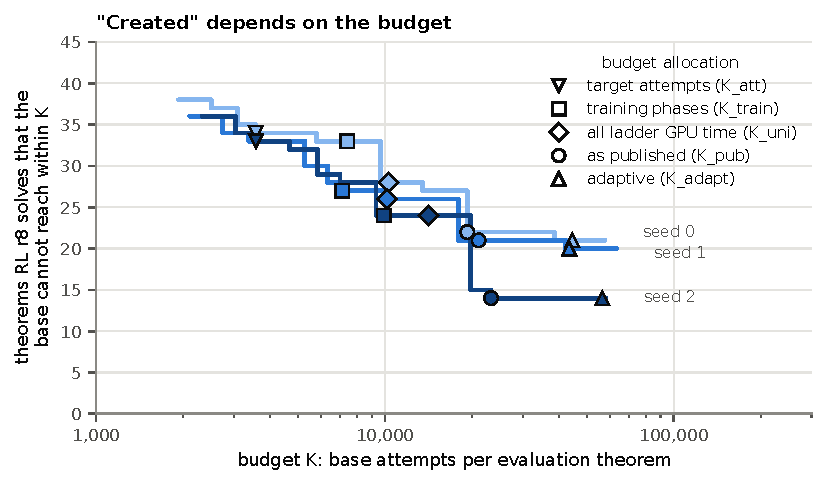
\includegraphics[width=0.66\linewidth]{figures/fig4_budget.pdf}
\caption{The compute-matched ``created'' set (RL r8 solves, the base cannot reach within $K$) against the base budget
$K$, for full-exposure seeds s0--s2. Markers are the five budget allocations of Table~\ref{tab:budgets}. Lines end
where the base data stop deciding membership.}
\label{fig:budget}
\end{figure}

\paragraph{$k$-to-solve intervals and the known-proof estimator.} Sampling gives $\hat p = c/n$ and a one-sided 95\%
Clopper--Pearson upper bound \ub{}. For rare events we add a lower estimate from likelihoods. The \emph{known-proof
estimate} $E(t)$ sums, over every Lean-accepted proof of $t$ that any model found, the base's teacher-forced probability
of that proof at $T=0.8$. The sum also runs over the environment's 33 naming offsets. The interval
$[1/\ub,\ 1/E]$ brackets the $k$-to-solve. $E$ is not a strict lower bound, because the sampler conditions on its own
names and unseen proofs are missing, so we calibrated it against large-$k$ sampling (Fig.~\ref{fig:estimator}). On
calibration theorems with 3--100 successes in 512, it recovers a median 0.98/0.94/0.93 of the measured $p$. Across 196
(seed, theorem) pairs with large-$k$ sampling, the median of $E/\hat p$ is 0.937 for $\hat p \geq 10^{-3}$ (106 pairs),
0.883 for $10^{-4}$--$10^{-3}$ (52), and 0.454 for $10^{-5}$--$10^{-4}$ (36). The estimate is usable in aggregate down
to about $10^{-4}$. Below that it runs about two-fold low, so a ``within reach if $E \geq 2/K$'' rule loses power
exactly where RL's budgets sit ($K \approx 10^4$). Sampling verdicts stay primary.

\paragraph{Certificates.} A theorem is \emph{certified out of reach at $K$} if $\ub < 0.05/K$. With zero successes
this needs about $60K$ attempts. We sampled the base 1.1--1.5 million times on 9 (theorem, seed) pairs from the
compute-matched sets: 7 of 9 certify at $\Kpub$. A pair \emph{survives every RL-free control} if it also has no success
from the replay-only control, from the compute-matched pretraining continuation, or from any other seed's base. Four
pairs on three theorems survive at $\Kpub$. Only one of the three theorems, a Peirce instance, is classical-only. Their
known proofs bound the base's $k$-to-solve from above at $10^{10}$--$10^{13}$. That is an extrapolation far outside
the estimator's calibrated range; sampling shows only $>4\times 10^5$.

\paragraph{RL-free controls.} Two controls receive RL's training without RL's proofs. The \emph{replay-only} control
fine-tunes pend for the same eight rounds on pretraining replay alone. It solves 239/244/249 of the 322, against pend's
232/236/234 and r8's 286/286/293. The \emph{continuation} control trains pend further on \KT{} for about 75--78\% of the
ladder's GPU time (same-class seconds). It solves 220/215/219: it gains 12--19 theorems and loses 30--42. At matched
gains in IRT ability, EI flags no more items as differentially improved than replay-only training. The weight update
of eight RL rounds is about as large as replay-only's (relative norm 0.28 vs 0.30, one seed). Twelve operational
definitions of ``created'' agree poorly: the mean pairwise Jaccard similarity of their sets is 0.29 at r8 and 0.34
at r16. Different seeds' RL ``creates'' different theorems.

\paragraph{Exact likelihoods along RL.} For theorems that RL newly solves, the worst step of r8's eventual proof rises
under teacher forcing (at $T=1$) from about $-6.2$ nats at pend to about $-1.3$ at r8, mostly by round 4. RL also lifts the
pretraining reference proofs of these theorems, about three times less. For theorems that neither pend nor r8 solves,
the reference proofs do not improve under RL. The likelihood view agrees with the budget view. RL concentrates
probability on proofs whose hardest step the base already rated within a few nats.

\paragraph{From measurement to intervention.} Every criterion above compares a model with its own base. The base
always \emph{could} have written the proof with some small probability, so each criterion only bounds that probability
from above at some budget. The knockout below changes the base itself.

\paragraph{The knockout decision rule (pre-registered).} A family is \emph{acquired} (at the bar) by a model if the
model solves at least 50\% of the family's strict held-out members in a plain read of 256 attempts. Per family, the
verdicts were fixed before the ladders ran:
\begin{itemize}
\item \emph{created}: at least 2 of 6 knockout seeds acquire the family at r16, and the knockout base is certified out
of reach on it;
\item \emph{needs exposure}: at most one knockout seed acquires it, and the full arm acquires it on more seeds
(one-sided Boschloo test, $p \leq 0.05$);
\item \emph{neither}: no seed acquires it;
\item \emph{undetermined}: any other outcome.
\end{itemize}
The primary test compares, per seed, the indicator ``at least one family at the bar at r16'' between the full and
knockout arms. With six seeds per arm, the test rejects at full/knockout acquisitions of $(3,0)$, $(5,1)$ or $(6,2)$.
An outcome of 0/6 knockout seeds bounds the per-seed creation rate below 0.39 (one-sided 95\%).
